%\newpage
%\vspace{-3.0pt}
\section{Background}
\label{sec:background}
%\guy{Can someone check Sections 3-4-5? Especially the formulations}


%\subsection{Background}
%\label{subsec:background}

%\textbf{Petri nets.} 
\subsection{Petri Nets}
A Petri net $N$ is defined as a five-tuple $N=(P,T,\mathsf{pre},\mathsf{post},M_0)$ with $P$ being a set of places, $T$ being a set of transitions, $\mathsf{pre},\mathsf{post}:T\to\mathbb N^P$ being flow functions, and  $M_0\in\mathbb N^P$ being an initial distribution (a.k.a. \textit{marking}) of tokens in places.  
Transition $t$ is said to be \textit{enabled} at marking $M \in \mathbb N^P$ iff coordinate-wise it holds that $M\ge \mathsf{pre}(t)$, i.e., marking $M$ has at least as many tokens as is required by the flow function $\mathsf{pre}(t)$.
%
A transition \(t\) that is enabled may or may not \textit{fire}. If it fires, it consumes tokens based on $\mathsf{pre}(t)$, and produces tokens based on $\mathsf{post}(t)$. Firing a transition results in a new marking $M'$ (denoted as $M\xrightarrow{t}M'$), and with $M'= M - \mathsf{pre}(t) + \mathsf{post}(t)$. Differently put, firing a transition consumes input tokens and produces output tokens.
%
A single firing can naturally be extended to a firing \textit{sequence} $\sigma = t_1\cdots t_k$ (denoted as $M \xrightarrow{\sigma} M'$), giving rise to a sequence of markings $M_0,\ldots,M_k$ such that $M=M_0$, $M'=M_k$, and for all $i$ it holds that $M_i \xrightarrow{t_{i}} M_{i+1}$. 
% 
We define the (possibly infinite) set $R(N)=\{M \mid \exists \sigma\in T^*. M_0 \xrightarrow{\sigma} M\}$ to include all the markings of the Petri net that are reachable from the initial marking $M_0$.
% 
Given a Petri net $N$ and a marking $M$, the \textit{reachability problem} asks  whether $M\in R(N)$. 
%
Specifically, in this work we focus on reachability of a linear-constraint formula $\mathcal {F}$ over tokens. The formula is \sat\ if there exists a reachable marking $M\in R(N)$ which satisfies the constraints of $\mathcal {F}$ (this is denoted as $M \models \mathcal {F}$); otherwise, the formula is said to be \unsat{}.
%
Surprisingly, the Petri net reachability problem is decidable even in the \textit{unbounded} case, in which the net's places may hold an arbitrary number of tokens~\cite{Ma81,Ko82,La92}. 

\medskip
\noindent
\textbf{Example: PN definition and reachability.} 
%
Observe the toy Petri net in Fig.~\ref{fig:toyPN}.

\begin{figure}[H]
	\centering
	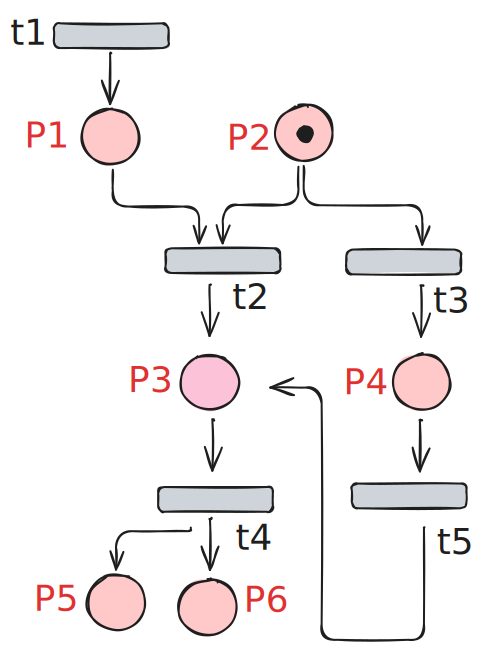
\includegraphics[width=0.3\textwidth]{plots/toy_PN_example.pdf}
	\caption{A toy Petri net.}
	\label{fig:toyPN}
\end{figure}



We formally define the net as follows:
%
\(N=(P,T,\mathsf{pre},\mathsf{post},M_0)\) with
\[
P=\{P_1,P_2,P_3,P_4,P_5,P_6\},\quad
T=\{t_1,t_2,t_3,t_4,t_5\},
\]
and the flow functions $\mathsf{pre}$,$\mathsf{post}$ are given as
\[
\begin{array}{c|cccccc}
	& P_1 & P_2 & P_3 & P_4 & P_5 & P_6 \\ \hline
	\mathsf{pre}(t_1)  & 0 & 0 & 0 & 0 & 0 & 0 \\
	\mathsf{post}(t_1) & 1 & 0 & 0 & 0 & 0 & 0 \\ \hline
	\mathsf{pre}(t_2)  & 1 & 1 & 0 & 0 & 0 & 0 \\
	\mathsf{post}(t_2) & 0 & 0 & 1 & 0 & 0 & 0 \\ \hline
	\mathsf{pre}(t_3)  & 0 & 1 & 0 & 0 & 0 & 0 \\
	\mathsf{post}(t_3) & 0 & 0 & 0 & 1 & 0 & 0 \\ \hline
	\mathsf{pre}(t_4)  & 0 & 0 & 1 & 0 & 0 & 0 \\
	\mathsf{post}(t_4) & 0 & 0 & 0 & 0 & 1 & 1 \\ \hline
	\mathsf{pre}(t_5)  & 0 & 0 & 0 & 1 & 0 & 0 \\
	\mathsf{post}(t_5) & 0 & 0 & 1 & 0 & 0 & 0
\end{array}
\]
The initial marking includes a single token in place $P_2$:
\[
M_0 = (0,1,0,0,0,0)^\top.
\]

%Differently put, there is .


\begin{itemize}
	\item An examples of a \emph{reachable} marking is
	\[
	M_f = (0,0,0,0,1,1)^\top,
	\]
	reached by the firing sequence
	\[
	M_0 \xrightarrow{t_1} M_1
	\xrightarrow{t_2} M_2
	\xrightarrow{t_4} M_f,
	\]
	where
	\[
	M_1 = (1,1,0,0,0,0)^\top,
	\quad
	M_2 = (0,0,1,0,0,0)^\top.
	\]
	\item An example of a \emph{non-reachable} marking is
	\[
	M_{nr} = (0,1,1,0,0,0)^\top.
	\]
	Since producing a token at \(P_3\) (via \(t_2\)) necessarily consumes the only token in \(P_2\) and, as no transition replenishes \(P_2\), it is impossible for these two places to \textit{simultaneously} hold a single token in any reachable firing. However, we note that if the initial marking were 
	
	\[
	M_0' = (0,2,0,0,0,0)^\top,
	\]
	then marking $M_{nr}$ \textit{would have} been reachable, by firing a single transition $t_1$, followed by a single transition $t_2$.
\end{itemize}



%\medskip
%\noindent
%\textbf{Verdict proofs.} 
\subsection{Verdict proofs}
If formula $\mathcal {F}$ is indeed \textit{reachable}, then there exists a witness sequence $\sigma\in T^*$ such that $M_0\xrightarrow{\sigma}M$ and also, $M\models \mathcal {F}$ serves as a proof that can be verified by simulating the Petri net firings.  
However, in the case that formula $\mathcal {F}$ is \textit{unreachable}, then there exists~\cite{Le09} a Presburger certificate $C$ that inductively proves non-reachability: 
(i) $M_0\models C$, (ii) $\forall t\in T \quad (M\models C \wedge M\xrightarrow{t}M')\Rightarrow M'\models C$, and (iii) $C\Rightarrow \neg \mathcal {F}$.

%\medskip
%\noindent
%\textbf{Semilinear sets and Parikh’s theorem.}

\subsection{Semilinear sets and Parikh’s theorem}
A set $S\subseteq\mathbb N^k$ is \textit{semilinear} if and only if it is a finite union of linear sets, i.e., for some $\mathbf b_i,\mathbf p_{i,j}\in\mathbb N^k$ it holds that:
\[S=\bigcup_{i=1}^m \{\mathbf b_i+\sum_{j=1}^{r_i} n_j\mathbf p_{i,j}\mid n_j\in\mathbb N\}.\]
Furthermore, semilinear sets coincide with sets that can be defined by \textit{Presburger arithmetic}~\cite{Pr29}. 
%
In the context of automata theory, Parikh’s theorem~\cite{Parikh66} proves that by applying the \textit{Parikh image} of any context-free language (CFL) --- we can obtain a semilinear set. 
%
The \emph{Parikh image} of a word $w$ over $\Sigma=\{a_1,\dots,a_k\}$ is defined as the vector:
\[
\mathsf{Parikh}(w)\;=\;\bigl(|w|_{a_1},\dots,|w|_{a_k}\bigr)\in\mathbb{N}^k,
\]
with $|w|_{a_i}$ counting occurrences of $a_i$ in $w$.
More generally, for a language $L\subseteq\Sigma^*$:
\[
\mathsf{Parikh}(L)\;=\;\{\mathsf{Parikh}(w)\mid w\in L\}\subseteq\mathbb{N}^k.
\]


%\medskip
%\noindent
%\textbf{Semilinear sets and Parikh’s theorem.} 
%A set $S\subseteq\mathbb N^k$ is \textit{semilinear} iff  
%$S=\bigcup_{i=1}^m \{\mathbf b_i+\sum_{j=1}^{r_i} n_j\mathbf p_{i,j}\mid n_j\in\mathbb N\}$,  
%for $\mathbf b_i,\mathbf p_{i,j}\in\mathbb N^k$.  
%Semilinear sets coincide with sets defined by \textit{Presburger arithmetic}~\cite{Pr29}.  
%By Parikh’s theorem~\cite{Parikh66}, the \textit{Parikh Image} of any context-free language is semilinear, with an effective construction.
%%
%For an alphabet $\Sigma=\{a_1,\dots,a_k\}$ and any word $w\in L\subseteq\Sigma^*$, the $\mathsf{Parikh}$ image is $\mathsf{Parikh}(w)=\{\,a_i^{|w|_{a_i}}\mid a_i\in\Sigma\,\}$, the multiset of symbols appearing in $w$ according to their number of occurrences.


%\med skip
%\noindent
%\textbf{Deciding serializability in unbounded systems.}
\subsection{Deciding serializability in unbounded systems}
Bouajjani et al.~\cite{BoEmEnHa13} have proved that, as a special case of \textit{bounded-barrier linearizability}, serializability in unbounded systems can be reduced to a Petri net reachability problem.

